\section{Experiments and Results}

We have carried out some simulations and experiments to confirm whether our learning process works.

\subsection{Opening a Garbage Bag}

First motion is to open a garbage bag by inflating with air. Since this motion requires enough speed to bring air in the bag, the motion trajectory has to be predefined with the speed configuration in order to apply it to the real robot which has a speed limitation on each joint. Therefore, it is suitable to use our learning process, which can reproduce the whole trajectory beforehand with the reference to the human demonstrations, also taking smoothness into account.

For human demonstration data, we used the time series data of the positions of both right and left hands referenced from the coordinate system defined on the face position.

\figref{open_garbage_bag_repro} shows the predicted HMM model and the output trajectories of the opening-a-garbage-bag motion.

\begin{figure}[htbp]
  \begin{center}
    \includegraphics[clip,width=7.0cm]{./figs/open_garbage_bag_repro.png}
    \caption{Reconstructed trajectory of opening a garbage bag using HMM parameters and solving LQR. Left and right figure shows position and velocity information respectively. Blue thick lines represent the reproduced trajectory. Red ellipsoids represent Gaussians which are estimated by HMM from human demonstrations, which is shown with thin colored lines (\( N = 4 \)). Note that the scale of each axis is normalized in positional space so that the scale can be ignored when estimating HMM parameters.}
    \label{figure:open_garbage_bag_repro}
  \end{center}
  \vspace{-3mm}
\end{figure}

\figref{open_garbage_bag_real} shows the snapshots of the real robot motion applying the reproduced trajectory above. The speed seemed to be fast enough to accomplish the task, comparing with the human. However, as a result, the bag didn't expand enough. The main reason seemed to be that the robot didn't use its wrists for now and so that it couldn't bring enough air into the bag. We are now working with that problem as one of the future works.

\begin{figure}[htbp]
  \begin{center}
    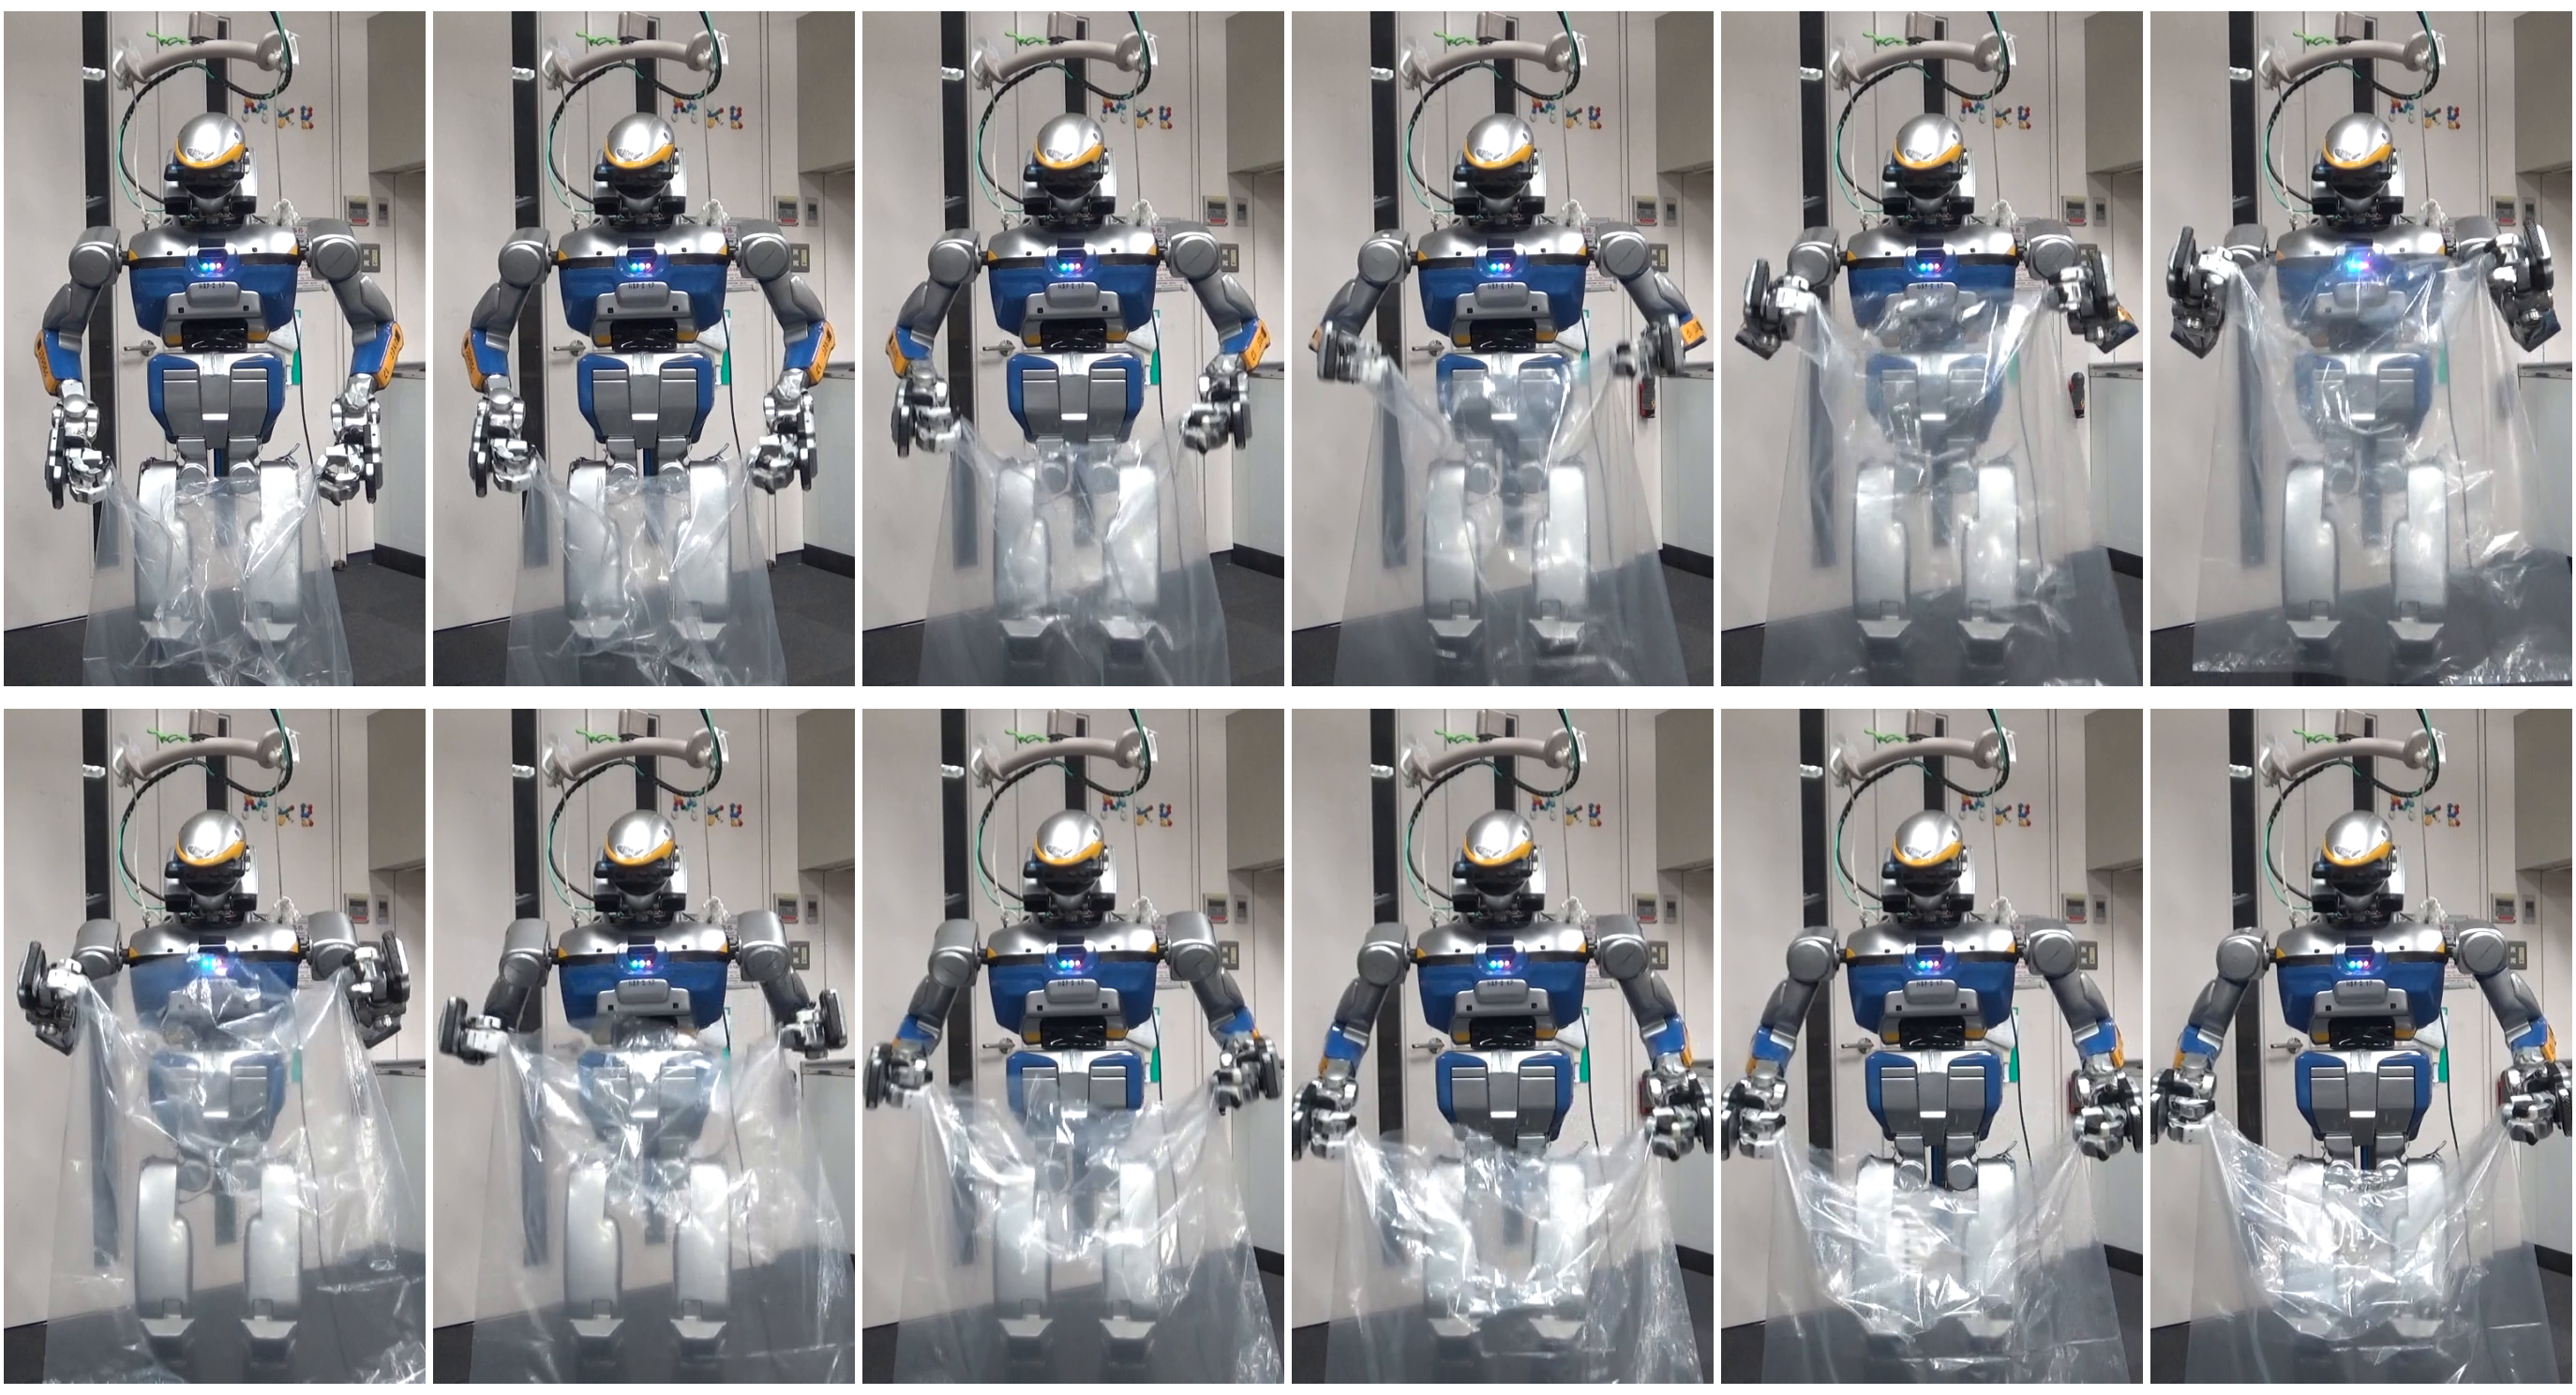
\includegraphics[clip,width=\linewidth]{./figs/open_garbage_bag_real.png}
    \caption{Snapshots of executing reproduced opening-a-garbage-bag trajectory with a humanoid robot. The result wasn't so efficient (the bag didn't expand enough), although the speed of the motion seemed to be fast enough. One reason might be the non-use of the wrists.}
    \label{figure:open_garbage_bag_real}
  \end{center}
\end{figure}

\subsection{Pushing buttons}

While the previous task, opening a garbage bag, has no target to approach or to touch, the target coordinates has to be considered when pushing buttons. We brought out an experimental environment, which is shown in the left figure in \figref{push_button}, and recorded some trajectories which reach the different buttons. As described in \subsecref{multi_coordinates}, we applied the multi coordinates version of HMM learning, whose two base coordinate systems are one set on the initial position and the other on the position of the target, which is the button here.

\begin{figure}[htbp]
  \begin{minipage}{0.40\hsize}
    \begin{center}
      \includegraphics[clip,width=\linewidth]{./figs/push_button.png}
    \end{center}
  \end{minipage}
  \begin{minipage}{0.60\hsize}
    \begin{center}
      \begin{minipage}{0.45\hsize}
        \begin{center}
          \includegraphics[clip,width=\hsize]{./figs/push_button_repro1.png}
        \end{center}
      \end{minipage}
      \begin{minipage}{0.45\hsize}
        \begin{center}
          \includegraphics[clip,width=\hsize]{./figs/push_button_repro2.png}
        \end{center}
      \end{minipage}
      \begin{minipage}{0.45\hsize}
        \begin{center}
          \includegraphics[clip,width=\hsize]{./figs/push_button_repro3.png}
        \end{center}
      \end{minipage}
      \begin{minipage}{0.45\hsize}
        \begin{center}
          \includegraphics[clip,width=\hsize]{./figs/push_button_repro4.png}
        \end{center}
      \end{minipage}
    \end{center}
  \end{minipage}
  \caption{Left: Experimental setup for collecting human demonstration data of pushing buttons. Buttons are aligned in the same plane. Right: Reproduced trajectory considering multi coordinate system when learning HMM. Yellow ellipsoids represent Gaussians which are the product of two Gaussians considering the initial coordinate system and the button coordinate system.}
  \label{figure:push_button}
\end{figure}

The right figures in \figref{push_button} show the reproduced trajectories whose initial positions are different from each other. Looking at the final position in each trajectory, it surely tend to reach the same position, which means the robot can reach each button correcty. We'll apply the trajectory into the real robot and confirm the accuracy.
